\documentclass[11pt]{article}
\usepackage[cm]{fullpage}
\usepackage{amsmath,amssymb}
\usepackage{graphicx}
\usepackage{color}
\usepackage{algorithm}
\usepackage{algcompatible}
\usepackage[relative,overlay]{textpos}
\usepackage[colorlinks,bookmarksopen,bookmarksnumbered,citecolor=red,urlcolor=red,breaklinks=true]{hyperref}
\newcommand{\cblue}[1]{{\color{blue}#1}}
\renewcommand{\vec}[1]{{#1}}
\newcommand{\figdir}{./figures/}
\newcommand{\note}[1]{\cblue{NOTE: #1}}
\author{Eike Mueller, University of Bath}
\date{\today}
\title{Multilevel Monte Carlo for Quantum Field Theories on the Lattice}
\begin{document}
\maketitle
%%%%%%%%%%%%%%%%%%%%%%%%%%%%%%%%%%%%%%%%%%%%%%%%%%%%%%%%%%%%%%%%%%%%%%%%%
\section{Motivation}
%%%%%%%%%%%%%%%%%%%%%%%%%%%%%%%%%%%%%%%%%%%%%%%%%%%%%%%%%%%%%%%%%%%%%%%%%
By using Feynman's path integral formulation of quantum mechanics \cite{Feynman2010}, lattice field theories predict the fundamental interactions of subatomic particles. Numerical results are obtained by Markov Chain Monte Carlo (MCMC) sampling of discretised fields on a space-time grid. To produce physically relevant results, both the number of lattice points and the number of Monte Carlo samples have to be increased, making accurate simulations prohibitively expensive. In similar contexts the Multilevel Monte Carlo (MLMC) algorithm \cite{Giles2015} has been shown to lead to a considerable reduction in computational complexity. The key idea is the construction of a set of coarse grained theories which accelerate sampling without introducing any additional bias errors. It should be stressed that MLMC is a proper variance reduction technique and goes beyond hierarchical samplers such as \cite{Faas1986}.
Recently the multilevel approach has been adapted to an MCMC setting in \cite{Dodwell2015}. We aim to apply the same methods in the context of lattice field theory, exploiting the natural hierarchy of coarse grained effectve theories obtained by renormalisation. In contrast to the Standard Monte Carlo (StMC) method, the computational complexity of MLMC is independent of the space-time dimension $d$. This makes the approach very promising for larger $d$, such as five-dimensional domain-wall fermion formulations \cite{Kaplan1992} of QCD. 
%%%%%%%%%%%%%%%%%%%%%%%%%%%%%%%%%%%%%%%%%%%%%%%%%%%%%%%%%%%%%%%%%%%%%%%%%
\section{Methods}
%%%%%%%%%%%%%%%%%%%%%%%%%%%%%%%%%%%%%%%%%%%%%%%%%%%%%%%%%%%%%%%%%%%%%%%%%

%%%%%%%%%%%%%%%%%%%%%%%%%%%%%%%%%%%%%%%%%%%%%%%%%%%%%%%%%%%%%%%%%%%%%%%%%
\subsection{Lattice Field Theory}
%%%%%%%%%%%%%%%%%%%%%%%%%%%%%%%%%%%%%%%%%%%%%%%%%%%%%%%%%%%%%%%%%%%%%%%%%
Let $\theta=\theta(x)$ the quantum field which is defined at any point $x$ in a $d$-dimensional box. The physically measurable expectation value $\langle Q\rangle$ of an observable (or ``quantity of interest'') $Q$ can be written as a sum over all possible field configurations $\theta$ weighted by the exponential of the action $S[\theta]$ (with normalisation factor $Z$):
\begin{equation}
  \langle Q\rangle = Z^{-1} \int_{\text{all $\theta$}} Q[\theta]e^{-S[\theta]} \approx \frac{1}{N} \sum_{n=1}^N Q[\theta_L^n] = \hat{Q}^{\text{StMC}}_{L,N} \qquad \mathbb{R}^{M}\ni \theta_L^n\sim e^{-S[\cdot]}
\end{equation}
In this equation two approximations are made to obtain an estimator $\hat{Q}^{\text{StMC}}_{L,N}$ for $\langle Q\rangle$:
\begin{itemize}
    \item \textbf{Discretisation}. The field $\theta$ is represented by its values $(\theta_L)_j$ at the $j=1,\dots,M=2^{L\cdot d}$ points of a $d$-dimensional space-time lattice with grid spacing $a=2^{-L}$. This introduces bias errors of $\mathcal{O}(a^\alpha)=\mathcal{O}(M^{-\alpha/d})$.
    \item \textbf{Stochastic integration}. The integral is evaluated by summing the value of the observables for $N$ random fields $\{\theta_L^n\}_{n=1}^N$ which are distributed according to $e^{-S[\cdot ]}$. The sampling error is $\propto{1/\sqrt{N}}$.
\end{itemize}
To control both errors the number of lattice sites $M$ and the number of MC samples $N$ have to be large. Sophisticated methods such as Hybrid Monte Carlo \cite{Duane1987} and improved actions \cite{Davies2004} have been developed to minimise those errors. The computational cost to reduce both below some tolerance $\epsilon$ is $\text{Cost}^{\text{StMC}}\propto M\cdot N=\mathcal{O}(\epsilon^{-2-d/\alpha})$.
%%%%%%%%%%%%%%%%%%%%%%%%%%%%%%%%%%%%%%%%%%%%%%%%%%%%%%%%%%%%%%%%%%%%%%%%%
\subsection{Multilevel Monte Carlo}
%%%%%%%%%%%%%%%%%%%%%%%%%%%%%%%%%%%%%%%%%%%%%%%%%%%%%%%%%%%%%%%%%%%%%%%%%
\begin{figure}
  \begin{center}
  \begin{minipage}{0.55\linewidth}
    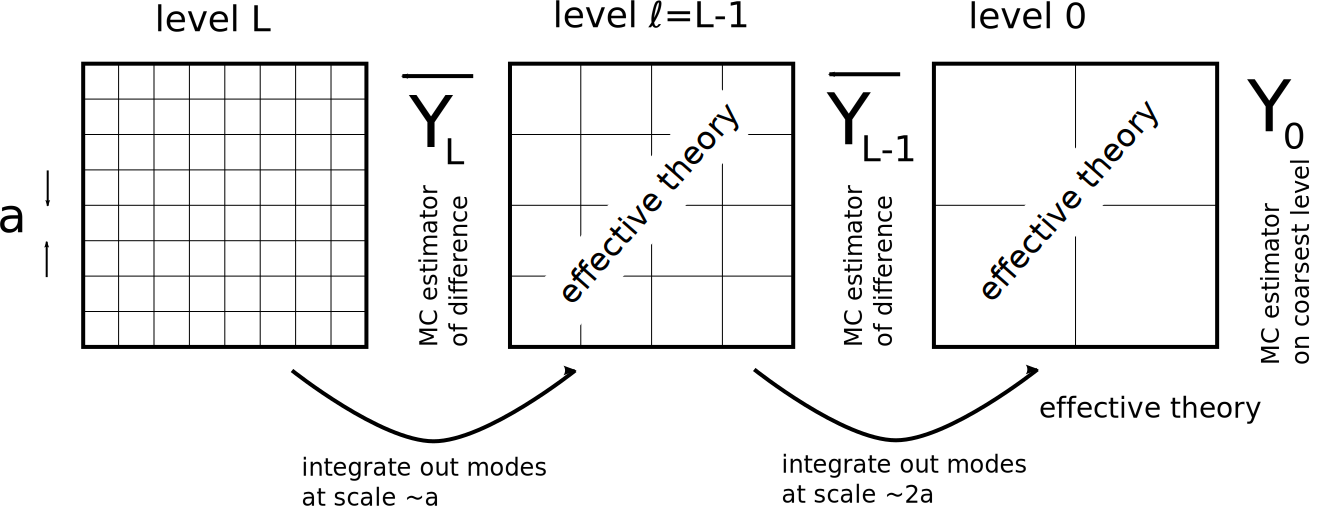
\includegraphics[width=\linewidth]{\figdir/multilevel_schematic.pdf}
  \end{minipage}
  \hfill
  \begin{minipage}{0.4\linewidth}
    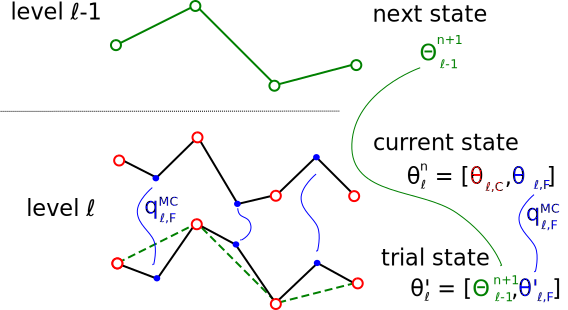
\includegraphics[width=\linewidth]{\figdir/multilevel_paths.pdf}
  \end{minipage}
  \caption{Multilevel hierarchy of grids (left) and hierarchical sampling of paths (right)}
  \end{center}
\end{figure}
Consider for example a one-dimensional quantum mechanical problem with quartic potential $V$. In this case the action is
\begin{equation}
  S\left[\theta_L\right] = \sum_{j=1}^M \frac{m_0}{2a}\left((\theta_L)_j-(\theta_L)_{j-1}\right)^2 + aV\left((\theta_L)_j\right)\qquad V(\theta) = \frac{1}{2}m_0\mu^2\theta^2+\frac{1}{4}\lambda^2\theta^4
\end{equation}
\begin{figure}
  \begin{center}
  \begin{minipage}{0.45\linewidth}
    \includegraphics[width=\linewidth]{\figdir/variance_decay_harmonic.pdf}
    \begin{textblock}{4.0}(1.25,-1.0)
      $V(\theta)=\frac{1}{2}\theta^2$
    \end{textblock}
    \begin{textblock}{4.0}(4.25,-2.75)
      \includegraphics[width=0.4\linewidth]{\figdir/potential_harmonic.pdf}
    \end{textblock}
  \end{minipage}
  \hfill
  \begin{minipage}{0.45\linewidth}
    \includegraphics[width=\linewidth]{\figdir/variance_decay_quartic.pdf}
    \begin{textblock}{4.0}(1.25,-1.0)
      $V(\theta)=-\frac{1}{2}\theta^2+\frac{1}{4}\theta^4$
    \end{textblock}
    \begin{textblock}{4.0}(4.25,-2.4)
      \includegraphics[width=0.4\linewidth]{\figdir/potential_quartic.pdf}
    \end{textblock}
  \end{minipage}
  \caption{Variance decay of difference estimator $Y_\ell$ between subsequent levels $\ell$ for the harmonic oscillator (left) and quartic double-well potential (right).}
  \end{center}
\end{figure}
\begin{equation}
  \hat{Q}_{L,\{N_\ell\}}^{\text{MLMC}} := \hat{Q}_{0,N_0}^{\text{StMC}} + \sum_{\ell=1}^L \hat{Y}_{\ell,N_\ell}^{\text{MC}}\qquad\text{with}\quad
  \hat{Y}_{\ell,N_\ell}^{\text{MC}} := \frac{1}{N_\ell}\sum_{n=1}^{N_\ell} \hat{Y}_\ell^n = \frac{1}{N_\ell}\sum_{n=1}^{N_\ell} \left(Q_\ell[\theta_\ell^n] - Q_{\ell-1}[\Theta_{\ell-1}^n]\right)
\end{equation}


%%%%%%%%%%%%%%%%%%%%%%%%%%%%%%%%%%%%%%%%%%%%%%%%%%%%%%%%%%%%%%%%%%%%%%%%%
\subsection{Effective Field Theories}
%%%%%%%%%%%%%%%%%%%%%%%%%%%%%%%%%%%%%%%%%%%%%%%%%%%%%%%%%%%%%%%%%%%%%%%%%


%%%%%%%%%%%%%%%%%%%%%%%%%%%%%%%%%%%%%%%%%%%%%%%%%%%%%%%%%%%%%%%%%%%%%%%%%
\section{Workplan}
%%%%%%%%%%%%%%%%%%%%%%%%%%%%%%%%%%%%%%%%%%%%%%%%%%%%%%%%%%%%%%%%%%%%%%%%%
\bibliographystyle{unsrt}
{\footnotesize
  \bibliography{plan}
}
\end{document}
